% !TEX program = xelatex
\documentclass[12pt]{article}
\usepackage[a4paper, margin=2.45cm]{geometry}
\usepackage[none]{hyphenat}
\usepackage[dvipsnames]{xcolor}
\usepackage[fleqn]{amsmath}
\usepackage{amssymb}
\usepackage{amsfonts}
\usepackage{graphicx}
\usepackage{cancel}
\usepackage{fontenc}
\usepackage{fontspec}
\usepackage{longtable}
\usepackage{listings}

\definecolor{bg}{gray}{0.1}
\setlength{\LTleft}{0pt}
\lstset{basicstyle = \footnotesize\color{white}\ttfamily, backgroundcolor = \color{bg}}
\AtBeginEnvironment{align}{\setcounter{equation}{0}}
\setmonofont{Consolas}
\sloppy
% \onehalfspacing
\newcommand{\tebal}[1]{\underline{\textbf{#1}}\bigskip}
\begin{document}

\noindent
2102800 - Muhammad Rahman Wicaksono - Pertemuan 11 Analisis Numerik\\
\noindent\rule{\textwidth}{0.2pt}\bigbreak

Sebuah percobaan memberikan nilai-nilai pada tabel berikut untuk peubah tak
bebasy untuk himpunan nilai-nilaix yang diberikan. Asumsuikan $y=f(x)$.
Lakukan pencocokan kuadrat terkecil yang sesuai untuk data berikut.
\begin{enumerate}
    \item {
        Soal no.1

        \begin{tabular}{|p{1cm}|p{1cm}|p{1cm}|p{1cm}|p{1cm}|p{1cm}|p{1cm}|p{1cm}|p{1cm}|p{1cm}|}
            \hline
            x & 1   & 2 & 3   & 4    & 5    & 6    & 7    & 8    & 9    \\ \hline
            y & 5.5 & 7 & 9.6 & 11.5 & 12.6 & 14.4 & 17.6 & 19.5 & 20.5 \\ \hline
        \end{tabular}

        Grafik ploting dari data tersebut adalah sebagai berikut
        \begin{center}
            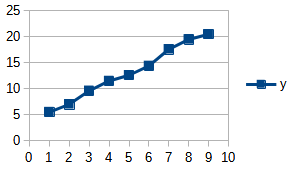
\includegraphics{grafik_1.png}
        \end{center}
        Terlihat bahwa ploting menyerupai grafik fungsi linier, sehingga dipiliih
        \begin{align*}
            f(x) = ax + b
        \end{align*}
        Maka diperoleh simpangan bakunya adalah
        \begin{align*}
            S   & = \sum_{i = 1}^9(y_i - f(x_i)) \\
                & = \sum_{i = 1}^9(y_i - ax_i - b)
        \end{align*}
        $ S $ bernilai minimun ketika $ \frac{\partial S}{\partial a} = 0 $ dan $ \frac{\partial S}{\partial b} = 0 $, sehingga diperoleh
        \begin{align*}
            0   & = \frac{\partial S}{\partial a}\\
            0   & = \cancel{-2}\sum_{i = 1}^{9}(y_i - ax_i - b)x_i\\
            0   & = \sum_{i = 1}^{9}y_ix_i - a\sum_{i = 1}^{9}x_i^{\;2} - b\sum_{i = 1}^{9}x_i \\
                & \Rightarrow a\sum_{i = 1}^{9}x_i^{\;2} + b\sum_{i = 1}^{9}x_i = \sum_{i = 1}^{9}y_ix_i
        \end{align*}
        \begin{align*}
            0   & = \frac{\partial S}{\partial b}\\
            0   & = \cancel{-2}\sum_{i = 1}^{9}(y_i - ax_i - b)\\
            0   & = \sum_{i = 1}^{9}y_i - a\sum_{i = 1}^{9}x_i - b\sum_{i = 1}^{9} \\
                & \Rightarrow a\sum_{i = 1}^{9}x_i + b\sum_{i = 1}^{9}1 = \sum_{i = 1}^{9}y_i
        \end{align*}
        Dari data awal dapat diperoleh
        \begin{align*}
            & \sum_{i = 1}^9x_i = 45 & 
            & \sum_{i = 1}^9x_i^{\;2} = 285 \\ 
            & \sum_{i = 1}^9y_i = 118,2 & 
            & \sum_{i = 1}^9y_ix_i = 707,4 \\
            & \sum_{i = 1}^91 = 9
        \end{align*}
        Maka diperoleh SPL sebagai berikut
        \begin{align*}
            \begin{matrix}
                285 a   & + & 45 b      & = 707,4 \\
                45 a    & + & 9 b       & = 118,2
            \end{matrix}
        \end{align*}
        Menggunakan program Gauss naif dari pertemeuan sebelumnya, diperoleh nilai $ a, b, c $ sebagai berikut
        \begin{lstlisting}

    Gauss Naif:
    a = 1.9399999999999995
    b = 3.4333333333333367
.
        \end{lstlisting}
        Maka diperoleh
        \begin{align*}
            f(x) = 1,9399999999999995x + 3.4333333333333367
        \end{align*}
        Diperoleh perbandingan grafik fungsi tersebut dengan ploting data awal adalah sebagai berikut
        \begin{center}
            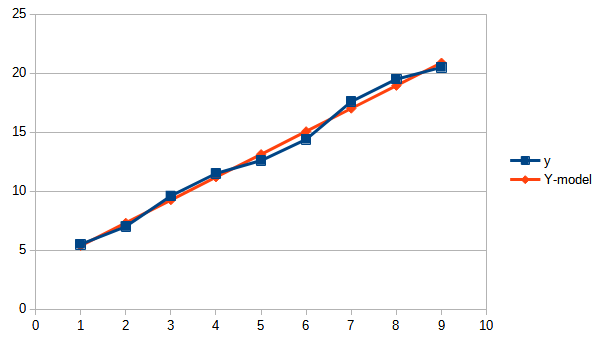
\includegraphics[scale=0.6]{hasil_1.png}
        \end{center}
    }
    \item {
        Soal no.4

        \begin{tabular}{|p{0.9cm}|p{0.9cm}|p{0.9cm}|p{0.9cm}|p{0.9cm}|p{0.9cm}|p{0.9cm}|p{0.9cm}|p{0.9cm}|p{0.9cm}|p{0.9cm}|}
            \hline
            x & 0.25 & 0.5 & 0.75 & 1    & 1.25 & 1.5  & 1.75 & 2    & 2.25 & 2.5  \\ \hline
            y & 3.1  & 1.7 & 1    & 0.68 & 0.42 & 0.26 & 0.14 & 0.09 & 0.04 & 0.03 \\ \hline
        \end{tabular}

        Grafik ploting dari data tersebut adalah sebagai berikut
        \begin{center}
            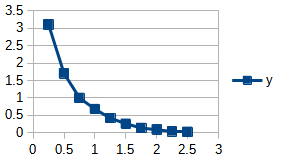
\includegraphics{grafik_4.png}
        \end{center}
        Terlihat bahwa ploting menyerupai grafik fungsi eksponen, sehingga dipiliih
        \begin{align*}
            f(x) = be^{ax}
        \end{align*}
        Perhatikan bahwa
        \begin{align*}
            y       & = f(x) \\
            \ln(y)  & = \ln(f(x)) \\
                    & = \ln(be^{ax}) \\
                    & = ax + ln(b)
        \end{align*}
        Maka diperoleh simpangan bakunya adalah
        \begin{align*}
            S   & = \sum_{i = 1}^{10}(\ln(y_i) - \ln(f(x_i))) \\
                & = \sum_{i = 1}^{10}(\ln(y_i) - ax_i - \ln(b))
        \end{align*}
        $ S $ bernilai minimun ketika $ \frac{\partial S}{\partial a} = 0 $ dan $ \frac{\partial S}{\partial \ln(b)} = 0 $, sehingga diperoleh
        \begin{align*}
            0   & = \frac{\partial S}{\partial a}\\
            0   & = \cancel{-2}\sum_{i = 1}^{10}(\ln(y_i) - ax_i - \ln(b))x_i\\
            0   & = \sum_{i = 1}^{10}\ln(y_i)x_i - a\sum_{i = 1}^{10}x_i^{\;2} - \ln(b)\sum_{i = 1}^{10}x_i \\
                & \Rightarrow a\sum_{i = 1}^{10}x_i^{\;2} + \ln(b)\sum_{i = 1}^{10}x_i = \sum_{i = 1}^{10}\ln(y_i)x_i
        \end{align*}
        \begin{align*}
            0   & = \frac{\partial S}{\partial \ln(b)}\\
            0   & = \cancel{-2}\sum_{i = 1}^{10}(\ln(y_i) - ax_i - \ln(b))\\
            0   & = \sum_{i = 1}^{10}\ln(y_i) - a\sum_{i = 1}^{10}x_i - \ln(b)\sum_{i = 1}^{10} \\
                & \Rightarrow a\sum_{i = 1}^{10}x_i + \ln(b)\sum_{i = 1}^{10}1 = \sum_{i = 1}^{10}\ln(y_i)
        \end{align*}
        Dari data awal dapat diperoleh
        \begin{align*}
            & \sum_{i = 1}^{10}x_i = 13,75 & 
            & \sum_{i = 1}^{10}x_i^{\;2} = 24,0625 \\ 
            & \sum_{i = 1}^{10}\ln(y_i) = -12,0376985211429 & 
            & \sum_{i = 1}^{10}\ln(y_i)x_i = -27,2079380741985 \\
            & \sum_{i = 1}^{10}1 = 10
        \end{align*}
        Maka diperoleh SPL sebagai berikut
        \begin{align*}
            \begin{matrix}
                24,0625 a   & + & 13,75 b      & = -27,2079380741985 \\
                13,75 a    & + & 10 b       & = -12,0376985211429
            \end{matrix}
        \end{align*}
        Menggunakan program Gauss naif dari pertemeuan sebelumnya, diperoleh nilai $ a, b, c $ sebagai berikut
        \begin{lstlisting}

    Gauss Naif:
    a = -2.0666380814791774
    ln(b) = 1.6378575099195791
.
        \end{lstlisting}
        Maka
        \begin{align*}
            a & = -2,0666380814791774 \\
            b & = 5,14413643604038
        \end{align*}
        Sehingga diperoleh
        \begin{align*}
            f(x) = 5,14413643604038e^{-2,0666380814791774x}
        \end{align*}
        Diperoleh perbandingan grafik fungsi tersebut dengan ploting data awal adalah sebagai berikut
        \begin{center}
            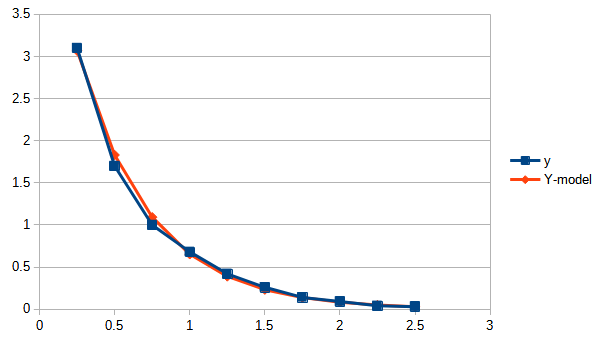
\includegraphics[scale=0.6]{hasil_4.png}
        \end{center}
    }
    \item {
        Soal no.5

        \begin{tabular}{|p{1cm}|p{1cm}|p{1cm}|p{1cm}|p{1cm}|p{1cm}|p{1cm}|p{1cm}|p{1cm}|p{1cm}|}
            \hline
            x & 0    & 0.2  & 0.4  & 0.6  & 0.8  & 1    & 1.2  & 1.4  & 1.6  \\ \hline
            y & 0.05 & 0.57 & 1.17 & 1.68 & 2.13 & 2.52 & 2.79 & 2.94 & 3.07 \\ \hline
        \end{tabular}
        \begin{tabular}{|p{1cm}|p{1cm}|p{1cm}|p{1cm}|p{1cm}|p{1cm}|p{1cm}|p{1cm}|p{1cm}|}
            \hline
            x & 1.8  & 2    & 2.2  & 2.4  & 2.6 & 2.8  & 3    & 3.2  \\ \hline
            y & 2.97 & 2.82 & 2.64 & 2.22 & 1.8 & 1.31 & 0.75 & 0.25 \\ \hline
        \end{tabular}

        Grafik ploting dari data tersebut adalah sebagai berikut
        \begin{center}
            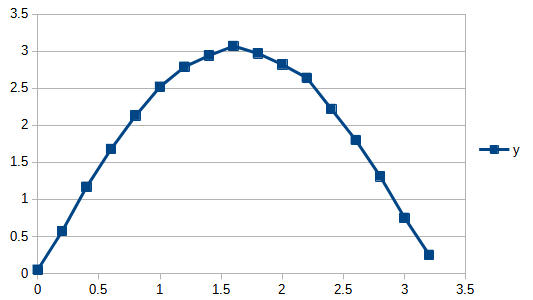
\includegraphics[scale=0.6]{grafik_5.png}
        \end{center}
        Terlihat bahwa ploting menyerupai grafik fungsi polinom derajat 2, maka dipiliih
        \begin{align*}
            f(x) = ax^2 + bx + c
        \end{align*}
        Maka diperoleh simpangan bakunya adalah sebagai berikut
        \begin{align*}
            S 
                & = \sum_{i = 1}^{17} (y_i - f(x_i))^2 \\
                & = \sum_{i = 1}^{17} (y_i - ax_i^{\;2} - bx_i - c)^2
        \end{align*}
        $ S $ bernilai minimun ketika $ \frac{\partial S}{\partial a} = 0, \frac{\partial S}{\partial b} = 0, \frac{\partial S}{\partial c} = 0 $, sehingga diperoleh
        \begin{align*}
            0   & = \frac{\partial S}{\partial a}\\
            0   & = \cancel{-2}\sum_{i = 1}^{17}(y_i - ax_i^{\;2} - bx_i - c)x_i^{\;2}\\
            0   & = \sum_{i = 1}^{17}y_ix_i^{\;2} - a\sum_{i = 1}^{17}x_i^{\;4} - b\sum_{i = 1}^{17}x_i^{\;3} - c\sum_{i = 1}^{17}x_i^{\;2} \\
                & \Rightarrow a\sum_{i = 1}^{17}x_i^{\;4} + b\sum_{i = 1}^{17}x_i^{\;3} + c\sum_{i = 1}^{17}x_i^{\;2} = \sum_{i = 1}^{17}y_i
        \end{align*}
        \begin{align*}
            0   & = \frac{\partial S}{\partial b}\\
            0   & = \cancel{-2}\sum_{i = 1}^{17}(y_i - ax_i^{\;2} - bx_i - c)x_i\\
            0   & = \sum_{i = 1}^{17}y_ix_i - a\sum_{i = 1}^{17}x_i^{\;3} - b\sum_{i = 1}^{17}x_i^{\;2} - c\sum_{i = 1}^{17}x_i \\
                & \Rightarrow a\sum_{i = 1}^{17}x_i^{\;3} + b\sum_{i = 1}^{17}x_i^{\;2} + c\sum_{i = 1}^{17}x_i = \sum_{i = 1}^{17}y_ix_i
        \end{align*}
        \begin{align*}
            0   & = \frac{\partial S}{\partial b}\\
            0   & = \cancel{-2}\sum_{i = 1}^{17}(y_i - ax_i^{\;2} - bx_i - c)\\
            0   & = \sum_{i = 1}^{17}y_i - a\sum_{i = 1}^{17}x_i^{\;2} - b\sum_{i = 1}^{17}x_i - c\sum_{i = 1}^{17}1 \\
                & \Rightarrow a\sum_{i = 1}^{17}x_i^{\;2} + b\sum_{i = 1}^{17}x_i + c\sum_{i = 1}^{17}1 = \sum_{i = 1}^{17}y_i
        \end{align*}
        Dari data awal dapat diperoleh
        \begin{align*}
            & \sum_{i = 1}^{17} 1            = 17 &
            & \sum_{i = 1}^{17} x_i          = 27,2 \\
            & \sum_{i = 1}^{17} x_i^{\;2}    = 59,84 &
            & \sum_{i = 1}^{17} x_i^{\;3}    = 147,968 \\
            & \sum_{i = 1}^{17} x_i^{\;4}    = 390,1568 &
            & \sum_{i = 1}^{17} y_i          = 31,68 \\
            & \sum_{i = 1}^{17} y_ix_i       = 51,71 &
            & \sum_{i = 1}^{17} y_ix_i^{\;2} = 100,5532 \\
        \end{align*}
        Maka diperoleh SPL sebagai berikut
        \begin{align*}
            \begin{matrix}
                390,1568 a &+& 147,968 b &+& 59,84 c    & = & 100,5532 \\
                147,968 a &+& 59,84 b &+& 27,2 c        & = & 51,71 \\
                59,84 a &+& 27,2 b &+& 17 c             & = & 31,68 
            \end{matrix}
        \end{align*}
        Menggunakan program Gauss naif dari pertemeuan sebelumnya, diperoleh nilai $ a, b, c $ sebagai berikut
        \begin{lstlisting}

    Gauss Naif:
    a = -1.1473490712074155
    b = 3.734139576883333
    c = -0.07242518059852361
.
        \end{lstlisting}
        Maka diperoleh
        \begin{align*}
            f(x) = -1,1473490712074155x^2 + 3,734139576883333x -0,07242518059852361
        \end{align*}
        Diperoleh perbandingan grafik fungsi tersebut dengan ploting data awal adalah sebagai berikut
        \begin{center}
            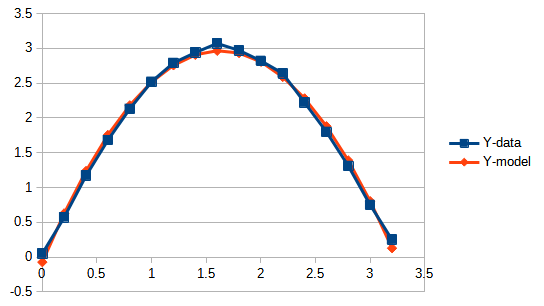
\includegraphics[scale=0.6]{hasil_5.png}
        \end{center}
        Perhatikan bahwa ploting data awal juga menyerupai fungsi trigonometri. Agar fungsi linier terhadap koefisien-koefisien yang akan dicari, maka dipiliih
        \begin{align*}
            f(x) = a\sin(x) + b 
        \end{align*}
        Maka dengan cara yang sama seperti sebelumnya, diperoleh
        \begin{align*}
            & a\sum_{i = 1}^{17}\sin^2(x_i) + b\sum_{i = 1}^{17}\sin(x_i) = \sum_{i = 1}^{17}y_i\sin(x_i)
        \end{align*}
        dan 
        \begin{align*}
            & a\sum_{i = 1}^{17}\sin(x_i) + b\sum_{i = 1}^{17}1 = \sum_{i = 1}^{17}y_i
        \end{align*}
        Dari data diperoleh
        \begin{align*}
            & \sum_{i = 1}^{17}1 = 17 & 
            & \sum_{i = 1}^{17}\sin(x_i) = 9,92895966988763 \\
            & \sum_{i = 1}^{17} = 7,85796495077195 &
            & \sum_{i = 1}^{17}y_i = 31,68 \\
            & \sum_{i = 1}^{17}y_i\sin(x_i) = 24,2807262974767
        \end{align*}
        Diperoleh SPL sebagai berikut
        \begin{align*}
            \begin{matrix}
                7,85796495077195a & + & 9,92895966988763b & = & 24,2807262974767 \\
                9,92895966988763a & + & 17b & = & 31,68
            \end{matrix}
        \end{align*}
        Solusi dari SPL tersebut adalah
        \begin{lstlisting}
            
    Gauss Naif:
    a = 2.8062753744875977
    b = 0.2245061755361081
.
        \end{lstlisting}
        Diperoleh
        \begin{align*}
            f(x) = 2,8062753744875977\sin(x) + 0,2245061755361081
        \end{align*}
        Grafik perbandingan antara fungsi dengan data diberikan sebagai berikut
        \begin{center}
            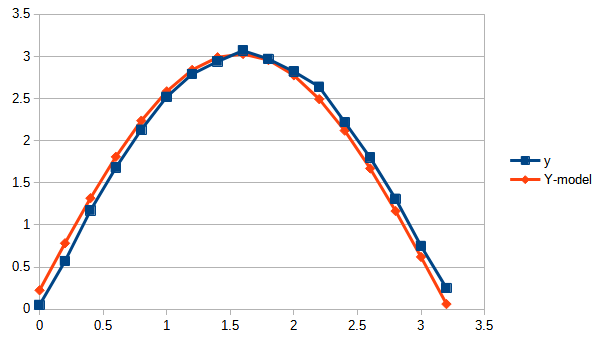
\includegraphics[scale=0.6]{hasil_5_b.png}
        \end{center}
    }
\end{enumerate}
\end{document}